 \documentclass[11pt]{article}
 \usepackage{graphicx}
 \usepackage{wrapfig}
 \usepackage{amssymb}
 \usepackage{lscape}
 \usepackage{times}
 
 \oddsidemargin=0.15in
 \evensidemargin=0.15in
 \textwidth=6.6in
 \textheight=9.3in
 \topmargin=0.in
 \footskip=0.6in
 
 \newcommand{\hbrk}{\hfill \break}
 
 
 \newcommand{\referenceA}{\rm }
 \newcommand{\referenceB}{\rm  }
 \newcommand{\referenceC}{\rm   }
 
 \pagestyle{myheadings}
 
 
 
 \begin{document}
 
 
 
 \mbox{\hspace{-.1\linewidth} 
 \begin{minipage}{0.6\linewidth} 
 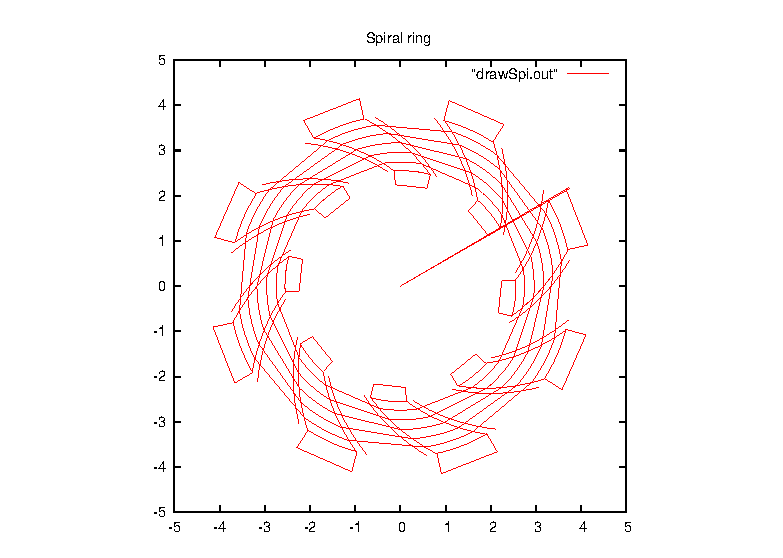
\includegraphics[width=9cm,height=9cm]{gnuplotRing.eps}
 \end{minipage}\hfill 
 \begin{minipage}{0.5\linewidth} 
   \begin{center}
   \large
     \begin{tabular}{lcl}
 Nb cells & 8 \\
 K &   3.50     \\
 $\xi$ &   50.0    & (deg.)  \\
 pf &  0.400     \\
 $r_1~/~r_2$  &   2.74     /    3.60    & (m)  \\
 $E_1~/~E_2$ &   17.0     /    180.    & (MeV)  \\
 $p_1~/~p_2$ &   179.     /    608.    & (MeV/c) \\
 $B\rho_1~/~B\rho_2$ &  0.598     /    2.03     &(T.m) \\
 Dip. sector angle &   18.0    & (deg.) \\
 Dip. bend angle &   45.0     & (deg.) \\
 Drift L, inj. &   1.29    -2$\times$0.15 & (m) \\
 Drift L, xtr. &   1.70    -2$\times$015 & (m) \\
     \end{tabular}
   \end{center}
 \end{minipage} 
 }
 
 \includegraphics[angle=-90,width=14cm]{mad.ps}
                                                                                                                                    
                                                                                                                                    
nCell    K         xi        Qx        Qy     MaxbetX   MaxBety    MaxDx                                                            
                                                                                                                                    
